\documentclass[a4paper]{article}
\usepackage[margin=1cm]{geometry}
\usepackage{amsmath, amssymb}
\usepackage{graphicx}
\usepackage{tikz}
\usetikzlibrary{arrows.meta}
\pagestyle{empty}

\definecolor{c0}{HTML}{E53935}
\definecolor{c1}{HTML}{1E88E5}
\definecolor{c2}{HTML}{43A047}
\definecolor{c3}{HTML}{FB8C00}
\definecolor{c4}{HTML}{8E24AA}
\definecolor{c5}{HTML}{00ACC1}
\definecolor{c6}{HTML}{F4511E}
\definecolor{c7}{HTML}{3949AB}
\definecolor{c8}{HTML}{7CB342}
\definecolor{c9}{HTML}{C2185B}
\definecolor{c10}{HTML}{FF7043}
\definecolor{c11}{HTML}{26A69A}
\definecolor{c12}{HTML}{5C6BC0}
\definecolor{c13}{HTML}{FFCA28}
\definecolor{c14}{HTML}{AB47BC}

\begin{document}

\begin{center}
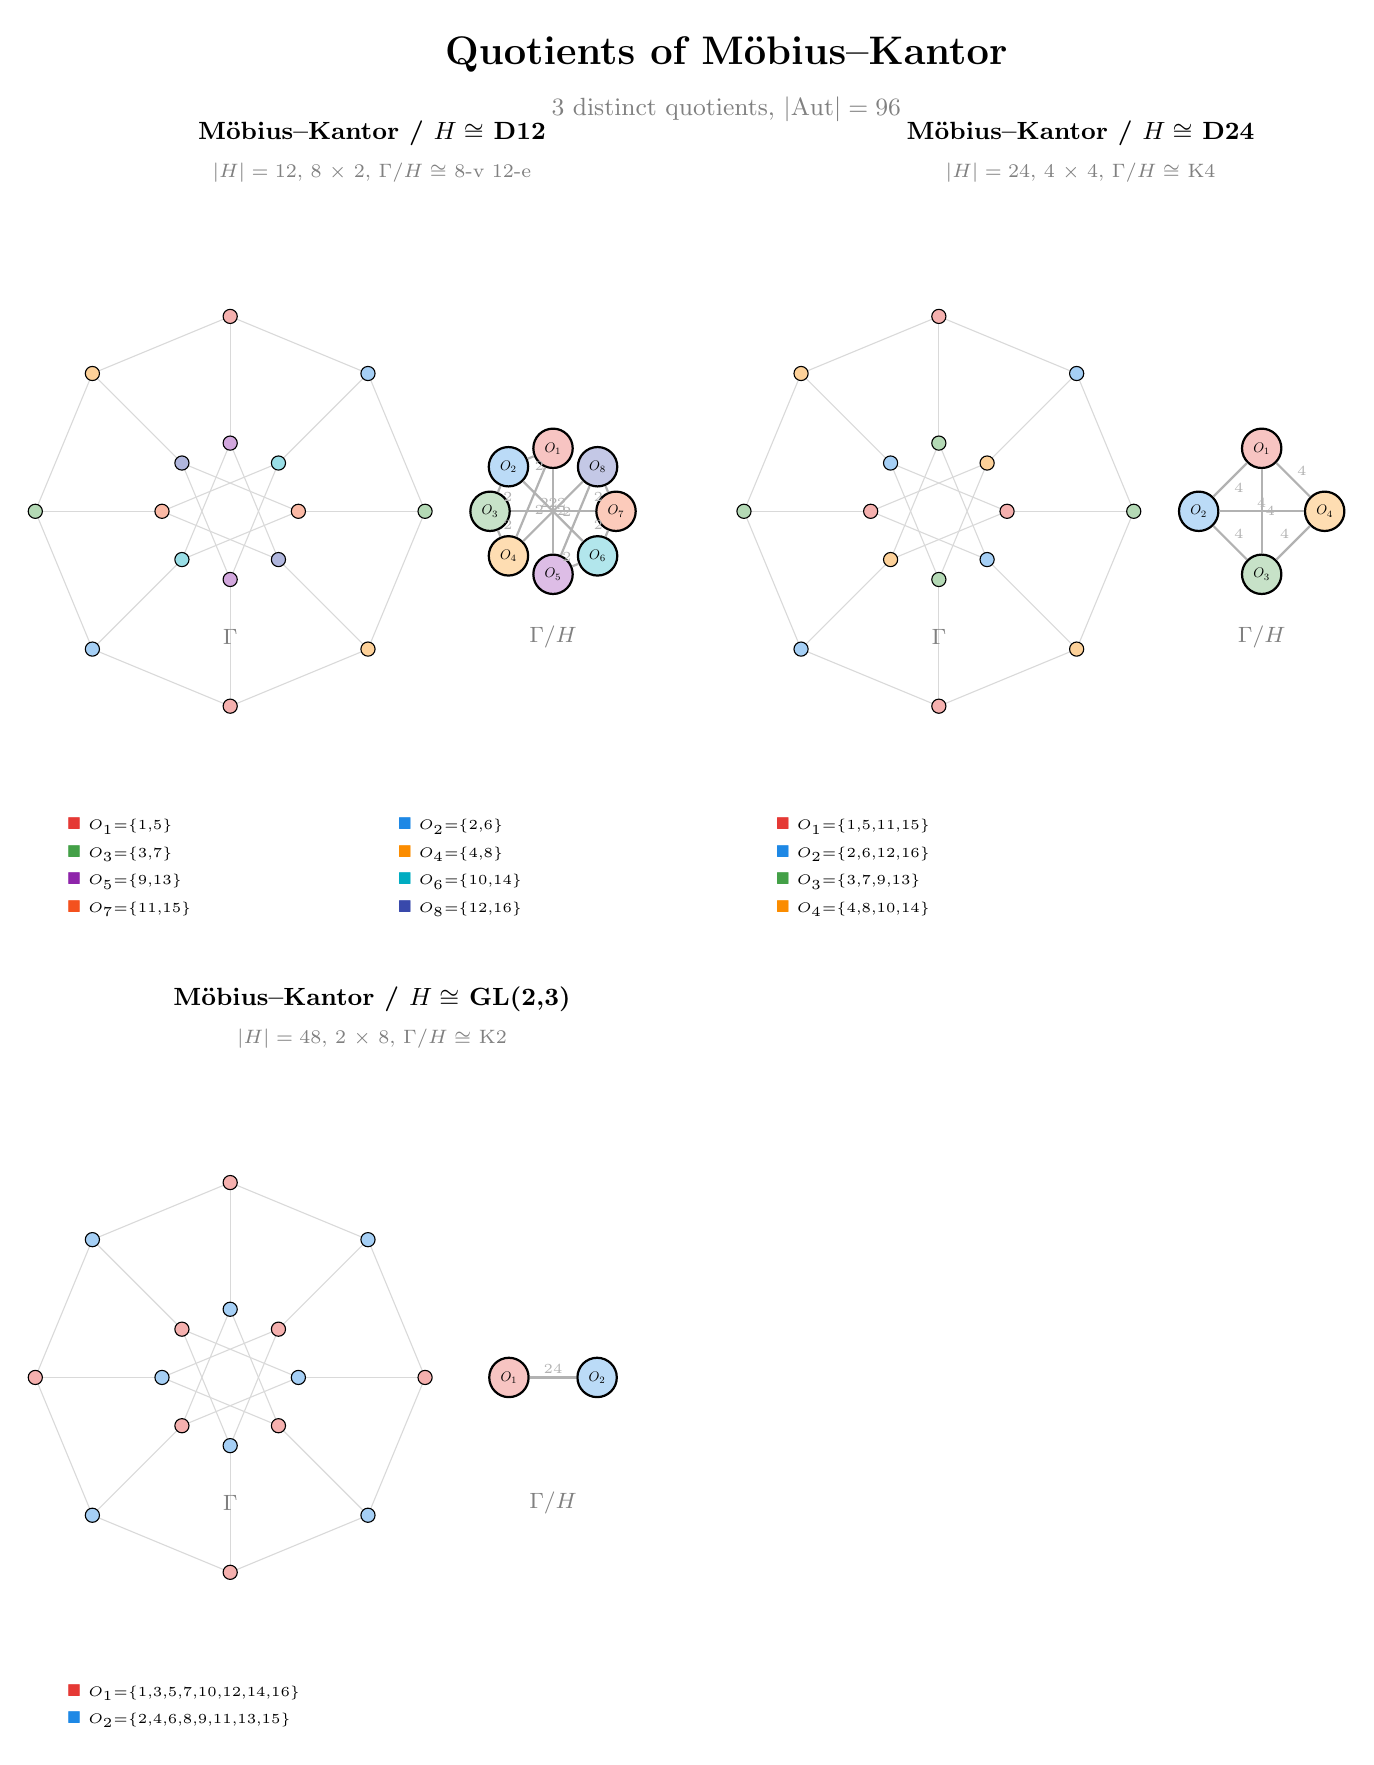
\begin{tikzpicture}[
  ov/.style={circle, draw, semithick, minimum size=3.5mm, inner sep=0pt},
  ovs/.style={circle, draw, thin, minimum size=1.8mm, inner sep=0pt},
  qv/.style={circle, draw, thick, minimum size=5mm, inner sep=0pt},
  cardtitle/.style={font=\small\bfseries},
  cardsub/.style={font=\scriptsize, text=gray},
  glabel/.style={font=\footnotesize, text=gray},
]
\node[font=\Large\bfseries] at (0, 11.5) {Quotients of M\"obius--Kantor};
\node[font=\small, text=gray] at (0, 10.8) {3 distinct quotients, $|\mathrm{Aut}|=96$};

% Card 1: H=D12
\node[cardtitle] at (-4.50,10.50) {M\"obius--Kantor / $H \cong$ D12};
\node[cardsub] at (-4.50,10.00) {$|H|=12$, 8 $\times$ 2, $\Gamma/H \cong$ 8-v 12-e};
\draw[gray!30, thin] (-6.300,8.175) -- (-4.550,7.450);
\draw[gray!30, thin] (-6.300,8.175) -- (-8.050,7.450);
\draw[gray!30, thin] (-6.300,8.175) -- (-6.300,6.566);
\draw[gray!30, thin] (-4.550,7.450) -- (-3.825,5.700);
\draw[gray!30, thin] (-4.550,7.450) -- (-5.687,6.313);
\draw[gray!30, thin] (-3.825,5.700) -- (-4.550,3.950);
\draw[gray!30, thin] (-3.825,5.700) -- (-5.434,5.700);
\draw[gray!30, thin] (-4.550,3.950) -- (-6.300,3.225);
\draw[gray!30, thin] (-4.550,3.950) -- (-5.687,5.087);
\draw[gray!30, thin] (-6.300,3.225) -- (-8.050,3.950);
\draw[gray!30, thin] (-6.300,3.225) -- (-6.300,4.834);
\draw[gray!30, thin] (-8.050,3.950) -- (-8.775,5.700);
\draw[gray!30, thin] (-8.050,3.950) -- (-6.913,5.087);
\draw[gray!30, thin] (-8.775,5.700) -- (-8.050,7.450);
\draw[gray!30, thin] (-8.775,5.700) -- (-7.166,5.700);
\draw[gray!30, thin] (-8.050,7.450) -- (-6.913,6.313);
\draw[gray!30, thin] (-6.300,6.566) -- (-5.687,5.087);
\draw[gray!30, thin] (-6.300,6.566) -- (-6.913,5.087);
\draw[gray!30, thin] (-5.687,6.313) -- (-6.300,4.834);
\draw[gray!30, thin] (-5.687,6.313) -- (-7.166,5.700);
\draw[gray!30, thin] (-5.434,5.700) -- (-6.913,5.087);
\draw[gray!30, thin] (-5.434,5.700) -- (-6.913,6.313);
\draw[gray!30, thin] (-5.687,5.087) -- (-7.166,5.700);
\draw[gray!30, thin] (-6.300,4.834) -- (-6.913,6.313);
\node[ovs, fill=c0!40] at (-6.300,8.175) {};
\node[ovs, fill=c1!40] at (-4.550,7.450) {};
\node[ovs, fill=c2!40] at (-3.825,5.700) {};
\node[ovs, fill=c3!40] at (-4.550,3.950) {};
\node[ovs, fill=c0!40] at (-6.300,3.225) {};
\node[ovs, fill=c1!40] at (-8.050,3.950) {};
\node[ovs, fill=c2!40] at (-8.775,5.700) {};
\node[ovs, fill=c3!40] at (-8.050,7.450) {};
\node[ovs, fill=c4!40] at (-6.300,6.566) {};
\node[ovs, fill=c5!40] at (-5.687,6.313) {};
\node[ovs, fill=c6!40] at (-5.434,5.700) {};
\node[ovs, fill=c7!40] at (-5.687,5.087) {};
\node[ovs, fill=c4!40] at (-6.300,4.834) {};
\node[ovs, fill=c5!40] at (-6.913,5.087) {};
\node[ovs, fill=c6!40] at (-7.166,5.700) {};
\node[ovs, fill=c7!40] at (-6.913,6.313) {};
\node[glabel] at (-6.30,4.10) {$\Gamma$};
\node[qv, fill=c0!30] (c0o0) at (-2.200,6.500) {\scalebox{0.5}{$O_{1}$}};
\node[qv, fill=c1!30] (c0o1) at (-2.766,6.266) {\scalebox{0.5}{$O_{2}$}};
\node[qv, fill=c2!30] (c0o2) at (-3.000,5.700) {\scalebox{0.5}{$O_{3}$}};
\node[qv, fill=c3!30] (c0o3) at (-2.766,5.134) {\scalebox{0.5}{$O_{4}$}};
\node[qv, fill=c4!30] (c0o4) at (-2.200,4.900) {\scalebox{0.5}{$O_{5}$}};
\node[qv, fill=c5!30] (c0o5) at (-1.634,5.134) {\scalebox{0.5}{$O_{6}$}};
\node[qv, fill=c6!30] (c0o6) at (-1.400,5.700) {\scalebox{0.5}{$O_{7}$}};
\node[qv, fill=c7!30] (c0o7) at (-1.634,6.266) {\scalebox{0.5}{$O_{8}$}};
\draw[gray!60, thick] (c0o0) -- node[font=\tiny, auto, inner sep=1pt] {2} (c0o1);
\draw[gray!60, thick] (c0o0) -- node[font=\tiny, auto, inner sep=1pt] {2} (c0o3);
\draw[gray!60, thick] (c0o0) -- node[font=\tiny, auto, inner sep=1pt] {2} (c0o4);
\draw[gray!60, thick] (c0o1) -- node[font=\tiny, auto, inner sep=1pt] {2} (c0o2);
\draw[gray!60, thick] (c0o1) -- node[font=\tiny, auto, inner sep=1pt] {2} (c0o5);
\draw[gray!60, thick] (c0o2) -- node[font=\tiny, auto, inner sep=1pt] {2} (c0o3);
\draw[gray!60, thick] (c0o2) -- node[font=\tiny, auto, inner sep=1pt] {2} (c0o6);
\draw[gray!60, thick] (c0o3) -- node[font=\tiny, auto, inner sep=1pt] {2} (c0o7);
\draw[gray!60, thick] (c0o4) -- node[font=\tiny, auto, inner sep=1pt] {2} (c0o5);
\draw[gray!60, thick] (c0o4) -- node[font=\tiny, auto, inner sep=1pt] {2} (c0o7);
\draw[gray!60, thick] (c0o5) -- node[font=\tiny, auto, inner sep=1pt] {2} (c0o6);
\draw[gray!60, thick] (c0o6) -- node[font=\tiny, auto, inner sep=1pt] {2} (c0o7);
\node[glabel] at (-2.20,4.10) {$\Gamma/H$};
\node[anchor=west, font=\tiny] at (-8.50,1.70) {\textcolor{c0}{$\blacksquare$} $O_{1}$=\{1,5\}};
\node[anchor=west, font=\tiny] at (-4.30,1.70) {\textcolor{c1}{$\blacksquare$} $O_{2}$=\{2,6\}};
\node[anchor=west, font=\tiny] at (-8.50,1.35) {\textcolor{c2}{$\blacksquare$} $O_{3}$=\{3,7\}};
\node[anchor=west, font=\tiny] at (-4.30,1.35) {\textcolor{c3}{$\blacksquare$} $O_{4}$=\{4,8\}};
\node[anchor=west, font=\tiny] at (-8.50,1.00) {\textcolor{c4}{$\blacksquare$} $O_{5}$=\{9,13\}};
\node[anchor=west, font=\tiny] at (-4.30,1.00) {\textcolor{c5}{$\blacksquare$} $O_{6}$=\{10,14\}};
\node[anchor=west, font=\tiny] at (-8.50,0.65) {\textcolor{c6}{$\blacksquare$} $O_{7}$=\{11,15\}};
\node[anchor=west, font=\tiny] at (-4.30,0.65) {\textcolor{c7}{$\blacksquare$} $O_{8}$=\{12,16\}};

% Card 2: H=D24
\node[cardtitle] at (4.50,10.50) {M\"obius--Kantor / $H \cong$ D24};
\node[cardsub] at (4.50,10.00) {$|H|=24$, 4 $\times$ 4, $\Gamma/H \cong$ K4};
\draw[gray!30, thin] (2.700,8.175) -- (4.450,7.450);
\draw[gray!30, thin] (2.700,8.175) -- (0.950,7.450);
\draw[gray!30, thin] (2.700,8.175) -- (2.700,6.566);
\draw[gray!30, thin] (4.450,7.450) -- (5.175,5.700);
\draw[gray!30, thin] (4.450,7.450) -- (3.313,6.313);
\draw[gray!30, thin] (5.175,5.700) -- (4.450,3.950);
\draw[gray!30, thin] (5.175,5.700) -- (3.566,5.700);
\draw[gray!30, thin] (4.450,3.950) -- (2.700,3.225);
\draw[gray!30, thin] (4.450,3.950) -- (3.313,5.087);
\draw[gray!30, thin] (2.700,3.225) -- (0.950,3.950);
\draw[gray!30, thin] (2.700,3.225) -- (2.700,4.834);
\draw[gray!30, thin] (0.950,3.950) -- (0.225,5.700);
\draw[gray!30, thin] (0.950,3.950) -- (2.087,5.087);
\draw[gray!30, thin] (0.225,5.700) -- (0.950,7.450);
\draw[gray!30, thin] (0.225,5.700) -- (1.834,5.700);
\draw[gray!30, thin] (0.950,7.450) -- (2.087,6.313);
\draw[gray!30, thin] (2.700,6.566) -- (3.313,5.087);
\draw[gray!30, thin] (2.700,6.566) -- (2.087,5.087);
\draw[gray!30, thin] (3.313,6.313) -- (2.700,4.834);
\draw[gray!30, thin] (3.313,6.313) -- (1.834,5.700);
\draw[gray!30, thin] (3.566,5.700) -- (2.087,5.087);
\draw[gray!30, thin] (3.566,5.700) -- (2.087,6.313);
\draw[gray!30, thin] (3.313,5.087) -- (1.834,5.700);
\draw[gray!30, thin] (2.700,4.834) -- (2.087,6.313);
\node[ovs, fill=c0!40] at (2.700,8.175) {};
\node[ovs, fill=c1!40] at (4.450,7.450) {};
\node[ovs, fill=c2!40] at (5.175,5.700) {};
\node[ovs, fill=c3!40] at (4.450,3.950) {};
\node[ovs, fill=c0!40] at (2.700,3.225) {};
\node[ovs, fill=c1!40] at (0.950,3.950) {};
\node[ovs, fill=c2!40] at (0.225,5.700) {};
\node[ovs, fill=c3!40] at (0.950,7.450) {};
\node[ovs, fill=c2!40] at (2.700,6.566) {};
\node[ovs, fill=c3!40] at (3.313,6.313) {};
\node[ovs, fill=c0!40] at (3.566,5.700) {};
\node[ovs, fill=c1!40] at (3.313,5.087) {};
\node[ovs, fill=c2!40] at (2.700,4.834) {};
\node[ovs, fill=c3!40] at (2.087,5.087) {};
\node[ovs, fill=c0!40] at (1.834,5.700) {};
\node[ovs, fill=c1!40] at (2.087,6.313) {};
\node[glabel] at (2.70,4.10) {$\Gamma$};
\node[qv, fill=c0!30] (c1o0) at (6.800,6.500) {\scalebox{0.5}{$O_{1}$}};
\node[qv, fill=c1!30] (c1o1) at (6.000,5.700) {\scalebox{0.5}{$O_{2}$}};
\node[qv, fill=c2!30] (c1o2) at (6.800,4.900) {\scalebox{0.5}{$O_{3}$}};
\node[qv, fill=c3!30] (c1o3) at (7.600,5.700) {\scalebox{0.5}{$O_{4}$}};
\draw[gray!60, thick] (c1o0) -- node[font=\tiny, auto, inner sep=1pt] {4} (c1o1);
\draw[gray!60, thick] (c1o0) -- node[font=\tiny, auto, inner sep=1pt] {4} (c1o2);
\draw[gray!60, thick] (c1o0) -- node[font=\tiny, auto, inner sep=1pt] {4} (c1o3);
\draw[gray!60, thick] (c1o1) -- node[font=\tiny, auto, inner sep=1pt] {4} (c1o2);
\draw[gray!60, thick] (c1o1) -- node[font=\tiny, auto, inner sep=1pt] {4} (c1o3);
\draw[gray!60, thick] (c1o2) -- node[font=\tiny, auto, inner sep=1pt] {4} (c1o3);
\node[glabel] at (6.80,4.10) {$\Gamma/H$};
\node[anchor=west, font=\tiny] at (0.50,1.70) {\textcolor{c0}{$\blacksquare$} $O_{1}$=\{1,5,11,15\}};
\node[anchor=west, font=\tiny] at (0.50,1.35) {\textcolor{c1}{$\blacksquare$} $O_{2}$=\{2,6,12,16\}};
\node[anchor=west, font=\tiny] at (0.50,1.00) {\textcolor{c2}{$\blacksquare$} $O_{3}$=\{3,7,9,13\}};
\node[anchor=west, font=\tiny] at (0.50,0.65) {\textcolor{c3}{$\blacksquare$} $O_{4}$=\{4,8,10,14\}};

% Card 3: H=GL(2,3)
\node[cardtitle] at (-4.50,-0.50) {M\"obius--Kantor / $H \cong$ GL(2,3)};
\node[cardsub] at (-4.50,-1.00) {$|H|=48$, 2 $\times$ 8, $\Gamma/H \cong$ K2};
\draw[gray!30, thin] (-6.300,-2.825) -- (-4.550,-3.550);
\draw[gray!30, thin] (-6.300,-2.825) -- (-8.050,-3.550);
\draw[gray!30, thin] (-6.300,-2.825) -- (-6.300,-4.434);
\draw[gray!30, thin] (-4.550,-3.550) -- (-3.825,-5.300);
\draw[gray!30, thin] (-4.550,-3.550) -- (-5.687,-4.687);
\draw[gray!30, thin] (-3.825,-5.300) -- (-4.550,-7.050);
\draw[gray!30, thin] (-3.825,-5.300) -- (-5.434,-5.300);
\draw[gray!30, thin] (-4.550,-7.050) -- (-6.300,-7.775);
\draw[gray!30, thin] (-4.550,-7.050) -- (-5.687,-5.913);
\draw[gray!30, thin] (-6.300,-7.775) -- (-8.050,-7.050);
\draw[gray!30, thin] (-6.300,-7.775) -- (-6.300,-6.166);
\draw[gray!30, thin] (-8.050,-7.050) -- (-8.775,-5.300);
\draw[gray!30, thin] (-8.050,-7.050) -- (-6.913,-5.913);
\draw[gray!30, thin] (-8.775,-5.300) -- (-8.050,-3.550);
\draw[gray!30, thin] (-8.775,-5.300) -- (-7.166,-5.300);
\draw[gray!30, thin] (-8.050,-3.550) -- (-6.913,-4.687);
\draw[gray!30, thin] (-6.300,-4.434) -- (-5.687,-5.913);
\draw[gray!30, thin] (-6.300,-4.434) -- (-6.913,-5.913);
\draw[gray!30, thin] (-5.687,-4.687) -- (-6.300,-6.166);
\draw[gray!30, thin] (-5.687,-4.687) -- (-7.166,-5.300);
\draw[gray!30, thin] (-5.434,-5.300) -- (-6.913,-5.913);
\draw[gray!30, thin] (-5.434,-5.300) -- (-6.913,-4.687);
\draw[gray!30, thin] (-5.687,-5.913) -- (-7.166,-5.300);
\draw[gray!30, thin] (-6.300,-6.166) -- (-6.913,-4.687);
\node[ovs, fill=c0!40] at (-6.300,-2.825) {};
\node[ovs, fill=c1!40] at (-4.550,-3.550) {};
\node[ovs, fill=c0!40] at (-3.825,-5.300) {};
\node[ovs, fill=c1!40] at (-4.550,-7.050) {};
\node[ovs, fill=c0!40] at (-6.300,-7.775) {};
\node[ovs, fill=c1!40] at (-8.050,-7.050) {};
\node[ovs, fill=c0!40] at (-8.775,-5.300) {};
\node[ovs, fill=c1!40] at (-8.050,-3.550) {};
\node[ovs, fill=c1!40] at (-6.300,-4.434) {};
\node[ovs, fill=c0!40] at (-5.687,-4.687) {};
\node[ovs, fill=c1!40] at (-5.434,-5.300) {};
\node[ovs, fill=c0!40] at (-5.687,-5.913) {};
\node[ovs, fill=c1!40] at (-6.300,-6.166) {};
\node[ovs, fill=c0!40] at (-6.913,-5.913) {};
\node[ovs, fill=c1!40] at (-7.166,-5.300) {};
\node[ovs, fill=c0!40] at (-6.913,-4.687) {};
\node[glabel] at (-6.30,-6.90) {$\Gamma$};
\node[qv, fill=c0!30] (c2o0) at (-2.760,-5.300) {\scalebox{0.5}{$O_{1}$}};
\node[qv, fill=c1!30] (c2o1) at (-1.640,-5.300) {\scalebox{0.5}{$O_{2}$}};
\draw[gray!60, thick] (c2o0) -- node[font=\tiny, auto, inner sep=1pt] {24} (c2o1);
\node[glabel] at (-2.20,-6.90) {$\Gamma/H$};
\node[anchor=west, font=\tiny] at (-8.50,-9.30) {\textcolor{c0}{$\blacksquare$} $O_{1}$=\{1,3,5,7,10,12,14,16\}};
\node[anchor=west, font=\tiny] at (-8.50,-9.65) {\textcolor{c1}{$\blacksquare$} $O_{2}$=\{2,4,6,8,9,11,13,15\}};
\end{tikzpicture}
\end{center}

\end{document}